\documentclass[11pt]{article}
\usepackage{fullpage}
\usepackage{setspace}
\usepackage{amsmath}
\usepackage{fancyvrb}
\usepackage{enumerate}
\usepackage{pgfplots}
\usepackage{graphicx}
\usepackage{float}
\usepackage{multirow}
\usepackage[format=hang,labelsep=quad]{caption}
\usepackage{subfig}
\usepackage{array}
\usepackage{multirow}

\renewcommand\thesubfigure{\roman{subfigure}}


\begin{document}
\noindent\large{Math 5365}\\
\large{Data Mining 1}\\
\large{Homework 17}\\
\large{Mary Barker}
\doublespace
\begin{enumerate}
\item 
 Generate a data set similar to the one displayed, where each of the 
 four clusters has 100 points.

\begin{center}
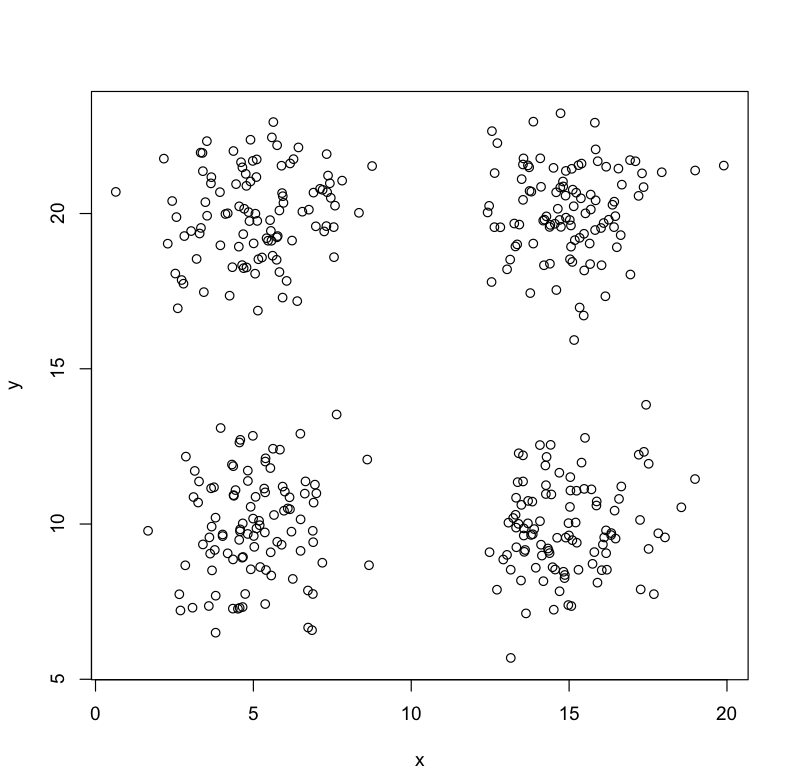
\includegraphics[scale=0.35]{pix/scatter_plot}
\end{center}

\begin{enumerate}
\item 
 Perform a K-means clustering with K = 4 and 1000 repetitions.

\item
 Plot the points and color them based on which clusters they are in.

\begin{center}
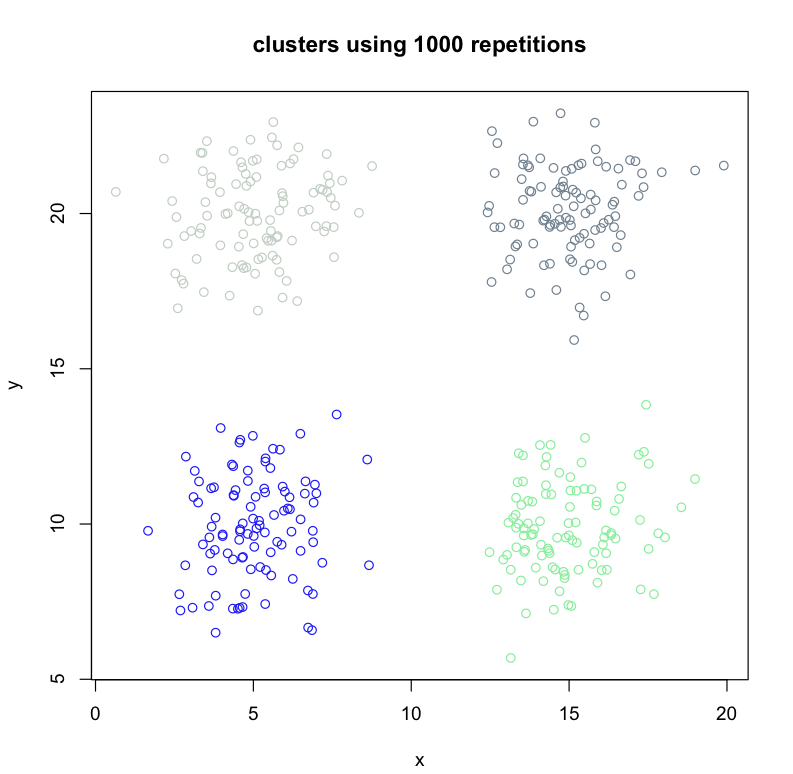
\includegraphics[scale=0.35]{pix/clustered}
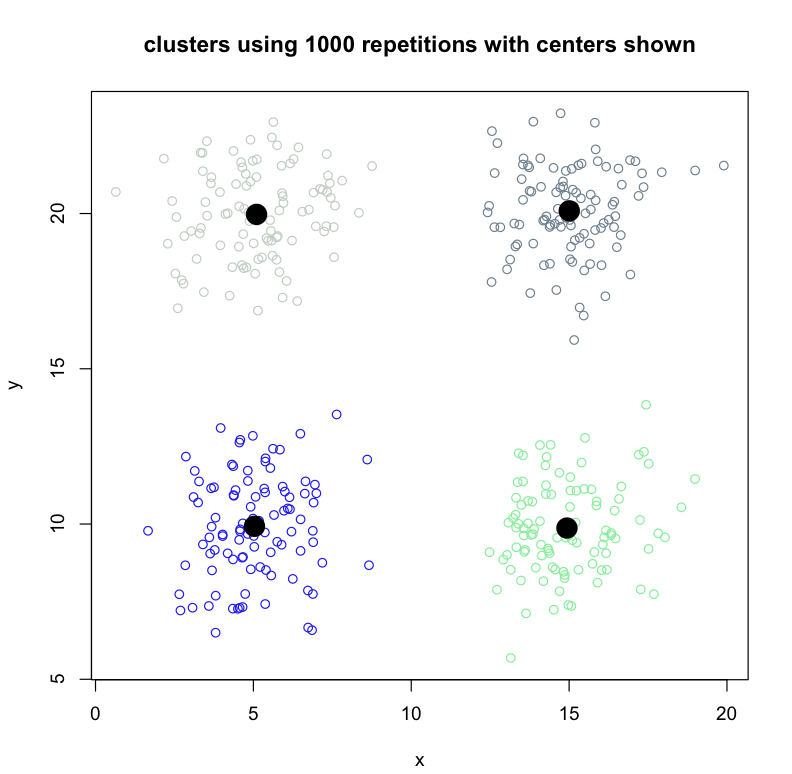
\includegraphics[scale=0.35]{pix/clustered_wcenters}
\end{center}

\item 
 Find the total, total within, and between sums of squares

The total sum of squares is 21777.85.

The total within sum of squares is 1711.74.

The total between sum of squares is 20066.11.

\item
 Find the centers of the clusters. 

The centers are in the table below

\begin{center}
\begin{tabular}{|c|c c|}
\hline
    &    x   &     y \\ \hline
1 &  5.034003 &  9.927154 \\
2 & 15.004838 & 20.085618 \\
3 & 14.931673 &  9.870831 \\
4 &  5.100832 & 19.972832 \\
\hline
\end{tabular}
\end{center}

\item 
 Suppose we want at least one of our repetitions of K-means to have 
 the property that every cluster contains exactly one initial centroid. 
 How many repetitions would be necessary to ensure that this happens 
 with at least 99\% probability? 

The minimum number of necessary repetitions is 47. 

\item 
 Can you find a choice of initial centers that does not result in the 
 optimal clusters? What is the total within sum of squares for that 
 clustering? 

The center of each cluster is ploted together with the colored points 
\begin{center}
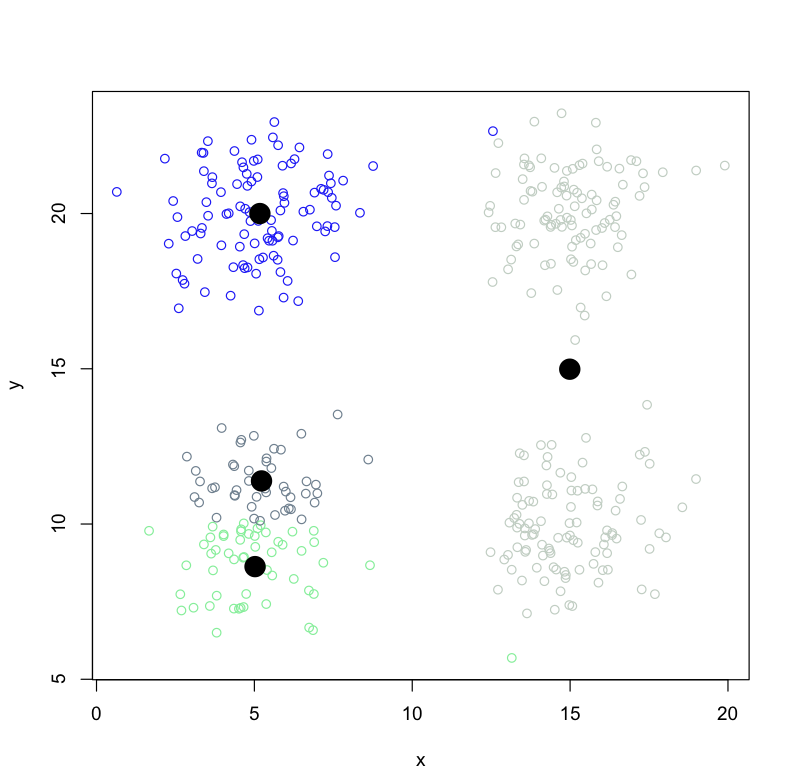
\includegraphics[scale=0.35]{pix/not_optimal}
\end{center}

The total within sum of squares for this case is 6728.091.
\end{enumerate}

\item 
 Perform a K-means clustering with K = 2 and 1000 repetitions for the 
 wdbc data set. What classification accuracy would be achieved if the 
 clusters were used to predict the diagnosis in this data set? 

The classification accuracy using K = 2 and 1000 repetitions is 
roughly 85.41301\%

\end{enumerate}
\begin{Verbatim}[numbers=left]
#Data Mining hw 17
library(stats)
wdbc <- read.csv('~/Dropbox/Tarleton/data_mining/dfiles/wdbc.data',
                 header=F,sep=',')
wdbc <- wdbc[,-1]
source('~/Dropbox/Tarleton/data_mining/generic_functions/dataset_ops.R')


# 1. Generate a data set similar to the one displayed, where each of the 
#    four clusters has 100 points.
set.seed(0)
x <- c(rnorm(100,  5, 1.5), rnorm(100, 15, 1.5), 
       rnorm(100,  5, 1.5), rnorm(100, 15, 1.5))
y <- c(rnorm(100, 10, 1.5), rnorm(100, 10, 1.5), 
       rnorm(100, 20, 1.5), rnorm(100, 20, 1.5))
plot(x, y)
points <- data.frame(x = x, y = y)

#   (a) Perform a K-means clustering with K = 4 and 1000 repetitions.

kmeans_reps <- function(dset, centers, reps){
  w_ss = Inf
  for(i in 1:reps){
    k_cluster <- kmeans(x = dset, centers = centers)
    if((k_cluster$tot.withinss) < w_ss){
      ssw = k_cluster$tot.withinss
      my_k_cluster <- k_cluster
    }
  }
  return(my_k_cluster)
}
reps = 1000
mycluster <- kmeans_reps(points, 4, reps)

#   (b) Plot the points and color them based on which clusters they are in.
plot(x, y, col=c('blue',
                'slategray',
                'lightgreen',
                'honeydew3',
                'orange',
                'brown')[mycluster$cluster],
                main='clusters using 1000 repetitions')
plot(x, y, col=c('blue',
                'slategray',
                'lightgreen',
                'honeydew3',
                'orange',
                'brown')[mycluster$cluster],
                main = 'clusters using 1000 repetitions with centers shown')
lines(mycluster$centers,type='p',pch=16,col='black', cex = 2.5)
#   (c) Find the total, total within, and between sums of squares
mycluster$totss
mycluster$tot.withinss
mycluster$betweenss

#   (d) Find the centers of the clusters. 
mycluster$centers

#   (e) Suppose we want at least one of our repetitions of K-means to have 
#       the property that every cluster contains exactly one initial centroid. 
#       How many repetitions would be necessary to ensure that this happens 
#       with at least 99% probability? 

minimum_reps <- function(k, err){
  ceiling(log(err) / log(1 - factorial(k) / (k^k)))
}
minimum_num = minimum_reps(4, 0.01)

#   (f) Can you find a choice of initial centers that does not result in the 
#       optimal clusters? What is the total within sum of squares for that 
#       clustering? 

# try with alternate centers:
centers04 <- cbind(c(10, 15, 10, 5), c(10, 15, 20, 15))
newcluster04 <- kmeans(x = points, centers = centers04)
plot(x, y, col=c('blue',
                'slategray',
                'lightgreen',
                'honeydew3',
                'orange',
                'brown')[newcluster04$cluster],
                main = 'clusters using 4 centers')
lines(newcluster04$centers,type='p',pch=16,col='black', cex = 2.5)

centers03 <- cbind(c(4, 15, 5, 16), c(10, 20, 10, 20))
newcluster03 <- kmeans(x = points, centers = centers03)
plot(x, y, col=c('blue',
                'slategray',
                'lightgreen',
                'honeydew3',
                'orange',
                'brown')[newcluster03$cluster],
                main = 'clusters using 4 centers')
lines(newcluster03$centers,type='p',pch=16,col='black', cex = 2.5)

centers02 <- cbind(c(5, 15, 15, 15), c(10, 15, 20, 12))
newcluster02 <- kmeans(x = points, centers = centers02)
plot(x, y, col=c('blue',
                'slategray',
                'lightgreen',
                'honeydew3',
                'orange',
                'brown')[newcluster02$cluster],
                main = 'clusters using 4 centers')
lines(newcluster02$centers,type='p',pch=16,col='black', cex = 2.5)

centers01 <- cbind(c(2, 10, 10, 20), c(2, 10, 20, 25))
newcluster01 <- kmeans(x = points, centers = centers01)
colors = 5 * c(1:50)
plot(x, y, col=c('blue',
                'slategray',
                'lightgreen',
                'honeydew3',
                'orange',
                'brown')[newcluster01$cluster],
                main = 'clusters using 4 centers')
lines(newcluster01$centers,type='p',pch=16,col='black', cex = 2.5)

# try with k = 1
newcluster1 <- kmeans(x = points, centers = 1)
plot(x, y, col=c('blue',
                'slategray',
                'lightgreen',
                'honeydew3',
                'orange',
                'brown')[newcluster1$cluster],
                main = 'clusters using 1 center')
lines(newcluster1$centers,type='p',pch=16,col='black', cex = 2.5)

# try with k = 2
newcluster2 <- kmeans(x = points, centers = 2)
plot(x, y, col=c('blue',
                'slategray',
                'lightgreen',
                'honeydew3',
                'orange',
                'brown')[newcluster2$cluster],
                main = 'clusters using 2 centers')
lines(newcluster2$centers,type='p',pch=16,col='black', cex = 2.5)

# try with k = 2
newcluster21 <- kmeans(x = points, centers = cbind(c(5, 16), c(10, 21)))
plot(x, y, col=c('blue',
                'slategray',
                'lightgreen',
                'honeydew3',
                'orange',
                'brown')[newcluster21$cluster],
                main = 'clusters using 2 centers')
lines(newcluster21$centers,type='p',pch=16,col='black', cex = 2.5)

# try with k = 6
newcluster6 <- kmeans(x = points, centers = 6)
plot(x, y, col=c('blue',
                'slategray',
                'lightgreen',
                'honeydew3',
                'orange',
                'brown',
                'yellow',
                'plum')[newcluster6$cluster],
                main = 'clusters using 6 centers')
lines(newcluster6$centers,type='p',pch=16,col='black', cex = 2.5)

# try with k = 8
newcluster8 <- kmeans(x = points, centers = 8)
plot(x, y, col=c('blue',
                'slategray',
                'lightgreen',
                'honeydew3',
                'orange',
                'brown',
                'yellow',
                'plum')[newcluster8$cluster],
                main = 'clusters using 8 centers')
lines(newcluster8$centers,type='p',pch=16,col='black', cex = 2.5)

# try with k = 10
newcluster10 <- kmeans(x = points, centers = 10)
plot(x, y, col=colors[newcluster10$cluster],
                main = 'clusters using 10 centers')
lines(newcluster10$centers,type='p',pch=16,col='black', cex = 2.5)

#brute force: 
d <- function(x1, x2){
  return(sqrt(sum( (x1 - x2)^2 )))
}
count = 1
list_of_clusters <- list()
keep_going = TRUE
for(i in 1:100000){
  if(keep_going){
    newcluster05 <- kmeans(x = points, centers = 4)
    plot(x, y, col=c('blue',
                    'slategray',
                    'lightgreen',
                    'honeydew3',
                    'orange',
                    'brown')[newcluster05$cluster])
    lines(newcluster05$centers,type='p',pch=16,col='black', cex = 2.5)
    x1 <- as.numeric(newcluster05$centers[1,])
    x2 <- as.numeric(newcluster05$centers[2,])
    x3 <- as.numeric(newcluster05$centers[3,])
    x4 <- as.numeric(newcluster05$centers[4,])
    mindist <- min(c(
      d(x1, x2), d(x1, x3), d(x1, x4), 
      d(x2, x3), d(x2, x4), 
      d(x3, x4)
    ))
    if(mindist < 5){
    	list_of_clusters[[count]] <- newcluster05
    	count = count + 1
    	keep_going = FALSE
    }
  }
}

# 2. Perform a K-means clustering with K = 2 and 1000 repetitions for the 
#    wdbc data set. What classification accuracy would be achieved if the 
#    clusters were used to predict the diagnosis in this data set? 

wdbc_cluster <- kmeans_reps(wdbc[,2:ncol(wdbc)], 2, 1000)
acc <- confmatrix(wdbc$V2, wdbc_cluster$cluster)
\end{Verbatim}

\end{document}
